\section{CEvent\-Loop  Class Reference}
\label{classCEventLoop}\index{CEventLoop@{CEvent\-Loop}}
{\tt \#include $<$CEvent\-Loop.h$>$}

Inheritance diagram for CEvent\-Loop::\begin{figure}[H]
\begin{center}
\leavevmode
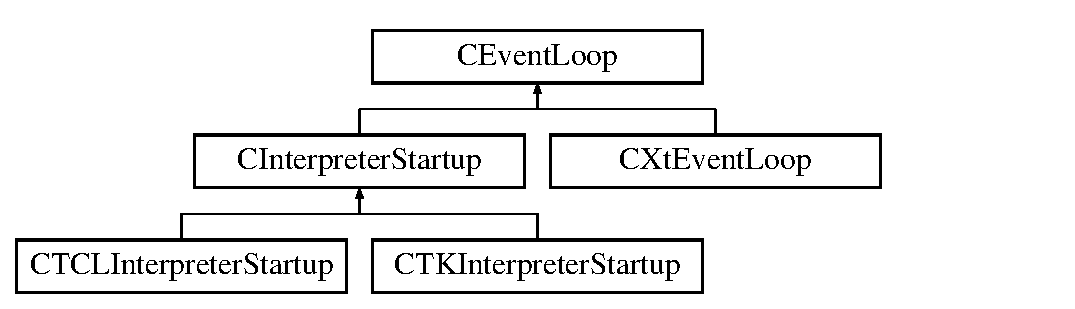
\includegraphics[height=3cm]{classCEventLoop}
\end{center}
\end{figure}
\subsection*{Public Methods}
\begin{CompactItemize}
\item 
{\bf CEvent\-Loop} ()
\item 
virtual {\bf $\sim$CEvent\-Loop} ()
\end{CompactItemize}
\subsection*{Static Public Methods}
\begin{CompactItemize}
\item 
CEvent\-Loop $\ast$ {\bf get\-Instance} ()
\end{CompactItemize}
\subsection*{Private Methods}
\begin{CompactItemize}
\item 
virtual int {\bf operator()} (int argc, char $\ast$$\ast$argv)=0
\begin{CompactList}\small\item\em Singleton instance.\item\end{CompactList}\item 
{\bf CEvent\-Loop} (const CEvent\-Loop \&a\-CEvent\-Loop)
\item 
CEvent\-Loop \& {\bf operator=} (const CEvent\-Loop \&a\-CEvent\-Loop)
\begin{CompactList}\small\item\em Not Implemented.\item\end{CompactList}\item 
int {\bf operator==} (const CEvent\-Loop \&a\-CEvent\-Loop) const
\begin{CompactList}\small\item\em Not Implemented.\item\end{CompactList}\end{CompactItemize}
\subsection*{Static Private Attributes}
\begin{CompactItemize}
\item 
CEvent\-Loop $\ast$ {\bf m\_\-p\-The\-Instance} = (CEvent\-Loop$\ast$)NULL
\end{CompactItemize}


\subsection{Detailed Description}
Encapsulates within a thread an application library which  runs it's own event loop. Examples are Xt and Tcl/Tk. These systems include their own mechanisms for detecting and dispatching events to application and framework specific code.

Attempting to instantiate more than one instance of an event  loop derived object results in a CDuplicate\-Singelton exception. Event loop derived processes implement operator() to  initiate an event loop how they are used depends on the iindividual framework. Each of these event loops is supposed to ensure that event dispatching to application level code is synchronized through the application's mutex. It is legal to synchronize all such events or an \char`\"{}appropriate subset\char`\"{}. 



Definition at line 315 of file CEvent\-Loop.h.

\subsection{Constructor \& Destructor Documentation}
\index{CEventLoop@{CEvent\-Loop}!CEventLoop@{CEventLoop}}
\index{CEventLoop@{CEventLoop}!CEventLoop@{CEvent\-Loop}}
\subsubsection{\setlength{\rightskip}{0pt plus 5cm}CEvent\-Loop::CEvent\-Loop ()}\label{classCEventLoop_a0}


The Constructs an event loop. Since event loops are singletons, this function throws a {\bf CDuplicate\-Singleton} {\rm (p.\,\pageref{classCDuplicateSingleton})} if the m\_\-p\-The\-Instance variable is not null. If the variable is null, it is filled in with this. 

Definition at line 323 of file CEvent\-Loop.cpp.

References m\_\-p\-The\-Instance.\index{CEventLoop@{CEvent\-Loop}!~CEventLoop@{$\sim$CEventLoop}}
\index{~CEventLoop@{$\sim$CEventLoop}!CEventLoop@{CEvent\-Loop}}
\subsubsection{\setlength{\rightskip}{0pt plus 5cm}CEvent\-Loop::$\sim$CEvent\-Loop ()\hspace{0.3cm}{\tt  [virtual]}}\label{classCEventLoop_a1}


The destructor sets the m\_\-p\-The\-Instance back to null. The assumption is that if derived classes catch the CDuplicate\-Singelton in their  constructors, they will re-throw it. Since such objects would be not fully constructed, they would not be destroyed and hence the instance pointer would not get spuriously deleted.



\begin{Desc}
\item[{\bf Bug: }]\par
There is no good way to enforce that {\bf CDuplicate\-Singleton} {\rm (p.\,\pageref{classCDuplicateSingleton})}'s don't result in spurious clears of the instance pointer.\end{Desc}
 

Definition at line 348 of file CEvent\-Loop.cpp.\index{CEventLoop@{CEvent\-Loop}!CEventLoop@{CEventLoop}}
\index{CEventLoop@{CEventLoop}!CEventLoop@{CEvent\-Loop}}
\subsubsection{\setlength{\rightskip}{0pt plus 5cm}CEvent\-Loop::CEvent\-Loop (const CEvent\-Loop \& {\em a\-CEvent\-Loop})\hspace{0.3cm}{\tt  [private]}}\label{classCEventLoop_c1}


Copy construction, assignment and comparison are not allowed. therefore they are declared as private and not implemented. 

\subsection{Member Function Documentation}
\index{CEventLoop@{CEvent\-Loop}!getInstance@{getInstance}}
\index{getInstance@{getInstance}!CEventLoop@{CEvent\-Loop}}
\subsubsection{\setlength{\rightskip}{0pt plus 5cm}CEvent\-Loop $\ast$ CEvent\-Loop::get\-Instance ()\hspace{0.3cm}{\tt  [static]}}\label{classCEventLoop_d0}


Retrieves the instance pointer. If the instance variable is null, throws CNo\-Such\-Object. 

Definition at line 365 of file CEvent\-Loop.cpp.

References m\_\-p\-The\-Instance.

Referenced by CTCLInterpreter\-Startup::Tcl\_\-Init(), and CTKInterpreter\-Startup::Tk\_\-Init().\index{CEventLoop@{CEvent\-Loop}!operator()@{operator()}}
\index{operator()@{operator()}!CEventLoop@{CEvent\-Loop}}
\subsubsection{\setlength{\rightskip}{0pt plus 5cm}virtual int CEvent\-Loop::operator() (int {\em argc}, char $\ast$$\ast$ {\em argv})\hspace{0.3cm}{\tt  [private, pure virtual]}}\label{classCEventLoop_c0}


Singleton instance.

Implemented by subclasses to provide the actual event loop functionality. int argc, char$\ast$$\ast$ argv provide a mechanism for passing parameters to the event loop thread as if it was run from a main program. 

Implemented in {\bf CInterpreter\-Startup} {\rm (p.\,\pageref{classCInterpreterStartup_c0})}, {\bf CTCLInterpreter\-Startup} {\rm (p.\,\pageref{classCTCLInterpreterStartup_c0})}, {\bf CTKInterpreter\-Startup} {\rm (p.\,\pageref{classCTKInterpreterStartup_c3})}, and {\bf CXt\-Event\-Loop} {\rm (p.\,\pageref{classCXtEventLoop_c0})}.\index{CEventLoop@{CEvent\-Loop}!operator=@{operator=}}
\index{operator=@{operator=}!CEventLoop@{CEvent\-Loop}}
\subsubsection{\setlength{\rightskip}{0pt plus 5cm}CEvent\-Loop\& CEvent\-Loop::operator= (const CEvent\-Loop \& {\em a\-CEvent\-Loop})\hspace{0.3cm}{\tt  [private]}}\label{classCEventLoop_c2}


Not Implemented.

\index{CEventLoop@{CEvent\-Loop}!operator==@{operator==}}
\index{operator==@{operator==}!CEventLoop@{CEvent\-Loop}}
\subsubsection{\setlength{\rightskip}{0pt plus 5cm}int CEvent\-Loop::operator== (const CEvent\-Loop \& {\em a\-CEvent\-Loop}) const\hspace{0.3cm}{\tt  [private]}}\label{classCEventLoop_c3}


Not Implemented.



\subsection{Member Data Documentation}
\index{CEventLoop@{CEvent\-Loop}!m_pTheInstance@{m\_\-pTheInstance}}
\index{m_pTheInstance@{m\_\-pTheInstance}!CEventLoop@{CEvent\-Loop}}
\subsubsection{\setlength{\rightskip}{0pt plus 5cm}CEvent\-Loop $\ast$ CEvent\-Loop::m\_\-p\-The\-Instance = (CEvent\-Loop$\ast$)NULL\hspace{0.3cm}{\tt  [static, private]}}\label{classCEventLoop_r0}


CEvent\-Loop$\ast$ m\_\-p\-The\-Instance Contains a pointer to the single event loop instance allowed. If there are no instances of the singleton, this pointer is null. Note that Get\-Instance will not attempt to create a new instance since it does not know which element of the class hierarchy to create. 

Definition at line 315 of file CEvent\-Loop.cpp.

Referenced by CEvent\-Loop(), and get\-Instance().

The documentation for this class was generated from the following files:\begin{CompactItemize}
\item 
{\bf CEvent\-Loop.h}\item 
{\bf CEvent\-Loop.cpp}\end{CompactItemize}
